\documentclass[11pt,largemargins]{h2wp}

\newcommand{\eventclass}{ریاضیات گسسته}
\newcommand{\eventtype}{افکار سازگار ، نوشتار نابکار}
\newcommand{\eventcntrbs}{سودابه محمدهاشمی - کیمیا محمدطاهری}

\begin{document}
\maketitle

هرگاه نویسنده‌ای توانایی درست نوشتن را نداشته باشد در انتقال صحیح تراوشات فکری خود به خواننده ناکام می‌ماند. نوشتار در خصوص مباحث علم ریاضیات گسسته نیز علاوه بر درک درست از مفاهیم، نیاز به دانش «صحیح نوشتن» و روش به تحریر درآوردن مسائل و اثبات‌ها دارد تا بتواند هدف انتقال بی‌ کم و کاست به خواننده را کسب نماید.

چیزی که واقعا اهمیت دارد این است که با درست نوشتن، خواننده درک صحیحی از راه و روش حل مسائل و اثبات‌ها كسب كند و توانایی درک و خلاقیت در کشف روش‌های حل مسائل را در خود ارتقاء بخشد.
در بیشتر مواقع اثبات مسائل آسان و منطق حل مسائل بسیار دست یافتنی به نظر می‌آید ولی در واقع در زمان نوشتن حل مسائل و اثبات‌ها رویکرد اشتباهی را پیش می‌گیریم.
به همین خاطر است که ما نیاز داریم یاد بگیریم كه چگونه اثبات‌ها را دنبال کنیم.

هر چند كه رعایت حداقل معیارهای درست نویسی و پیشبرد مرحله به مرحله‌ی حل مسائل و اثبات‌ها با استدلال‌های منطقی، خیال ما را نسبت به درست و معتبر بودن نوشته‌ی خود راحت می‌نماید ولی مطالعه‌ی متون فنی و تعمق در نوشتارهای غنیِ ما را به مرحله‌ای از بلوغ در نویسندگی می‌رساند كه علاوه بر رسیدن به بهترین نتیجه‌ی ممكن، ما را در انتقال صحیح معنا و مفهوم و درك صحیح نوشته بسیار موفق می‌سازد
و در نهایت زمانی که فرا بگیریم، چگونه با اتكا به استدلال‌های درست اثباتمان را کامل کنیم، به فهم عمیق‌تری از مسائل می‌رسیم.

پایه و بنیاد درست نویسی بسیار آسان است. تنها کافی است که دقت نماییم تا جملات استفاده شده به یکی از اشکال زیر باشد:

\begin{enumerate}
\item
خود فرض مسئله باشد.
\item
به صورت كاملا شفاف و واضح از جملات قبلی نتیجه شده باشد.
\item
درستی آن قبلا اثبات شده باشد.
\end{enumerate}

در این جزوه تمام سعی و کوشش ما بر این بوده است تا شما را بیشتر با «درست نویسی» و نکاتی که خواننده را به این جهت سوق دهد آشنا کنیم.
امید است كه فراگیری نكات «درست نویسی» در تمامی مراحل زندگی راهبر و راهنمای شما باشد.


\textbf{انواع نکات}

در این جزوه با سه دسته نکته مواجه هستیم:
\begin{enumerate}

\item
دسته $E$: نکات درست نویسی که رعایت نکردن آن باعث ناقص شدن اثبات و در نتیجه کسر نمره می شود.
\item
دسته $N$: نکات درست نویسی که رعایت کردن آن‌ها واجب نیست, امابه خوانایی راه حل, ابهام زدایی, پرهیز از تکرار و جلوگیری از خطا کمک می کنند.
\item
دسته $T$: دام های آموزشی و خطاهای رایج در حل سوالات.

\end{enumerate}

\chapter*{شمارش}

%% question 1

\question


سه مهره رخ متمایز و صفحه شطرنجی $8\times8$ داریم. به چند روش می‌توان این سه مهره را در سه خانه از این صفحه قرار داد به طوری که حداقل یک مهره وجود داشته باشد که توسط هیچ مهره‌ای تهدید نمی‌شود؟
\solution
  سوال را با اصل متمم حل می‌کنیم:
  
      -  کل حالات:
      
        \[64\times63\times62\]
      -  حالات نامطلوب: حالاتی که همه رخ‌ها تهدید بشوند.
      
         رخ اول برای قرار گیری در صفحه شطرنجی 64 حالت دارد, حال چون رخ اول باید تهدید بشود رخ دوم را باید در سطر یا ستون رخ اول قرار بدهیم که ۱۴ حالت دارد. چون رخ سوم هم باید تهدید بشود باید در سطر یا ستون یکی از رخ‌ها باشد که در مجموع شامل ۶ خانه در سطر یا ستون مشترک دو رخ قبلی و ۱۴ خانه در سطرها یا ستون‌های غیر مشترک دو رخ است. پس کل حالت‌ها برابر است با:
         
         \[64\times14\times20\]
-         حالات مطلوب: طبق اصل متمم برابر است با:
         \[64\times63\times62 - 64\times14\times20\]
\notes
\Tnote{n1}
نشمردن همه حالت‌ها: در اینجا تمام حالات نامطلوب محاسبه نشده است, زیرا این امکان وجود دارد که رخ اول توسط رخ دوم تهدید نشود و این حالت در نظر گرفته نشده است.
\Nnote{n2}
بهتر بود اشاره شود که به دلیل تمایز رخ‌ها چنین نتیجه‌ای گرفته شده است.

\solution
     -  کل حالات:
     
        \[64\times63\times62\]
      -  حالات نامطلوب: حالاتی که همه رخ‌ها تهدید بشوند.
      
         \[64\times7\times20\times2\]
-         حالات مطلوب: طبق اصل متمم برابر است با:
         \[64\times63\times62 - 64\times14\times20\]
\notes
\Nnote{n3}
نبود توضیحات کافی برای عبارت: به دلیل نبود توضیحات کافی, تشخیص چرایی غلط بودن جواب نهایی ممکن نیست.
\solution*{پاسخ صحیح}

   -  کل حالات: به دلیل تمایز رخ‌ها برابر است با:
   
        \[ P(64,3) = 64\times63\times62\]
      -  حالات نامطلوب: حالاتی که همه رخ‌ها تهدید بشوند.
      
      دو حالت داریم:
      \begin{enumerate}
\item
رخ اول رخ دوم را تهدید کند:

         رخ اول برای قرار گیری در صفحه شطرنجی 64 حالت دارد, حال چون رخ اول باید توسط رخ دوم تهدید بشود رخ دوم را باید در سطر یا ستون رخ اول قرار بدهیم که ۱۴ حالت دارد. چون رخ سوم هم باید تهدید بشود باید در سطر یا ستون یکی از رخ ها باشد که در مجموع شامل ۶ خانه در سطر یا ستون مشترک دو رخ قبلی و ۱۴ خانه در سطرها یا ستون‌های غیر مشترک دو رخ است. پس کل حالت‌ها برابر است با:
         
         \[64\times14\times20\]
\item
رخ اول رخ دوم را تهدید نکند:

         رخ اول برای قرار گیری در صفحه شطرنجی 64 حالت دارد, حال چون رخ اول نباید توسط رخ دوم تهدید بشود رخ دوم را در خانه‌ای به جز سطر یا ستون رخ اول قرار بدهیم که ۴۹ حالت دارد. حال رخ سوم باید هر دو رخ را تهدید کند پس باید در یکی از محل‌های تقاطع سطر و ستون رخ اول و رخ دوم قرار بگیرد که دو حالت دارد, پس کل حالت‌ها برابر است با:
         
         \[64\times49\times2\]
         
      \end{enumerate}
-         حالات مطلوب: طبق اصل متمم برابر است با:
         \[64\times63\times62\ - (64\times14\times20\ + 64\times49\times2\ )\]
  
%% question 2
       
\question


  اتحاد زیر را ثابت کنید.
  
     $$1^2 {n \choose 1} + 2^2 {n \choose 2} + 3^2 {n \choose 3} + ... + n^2 {n \choose n} = n(n+1)2^{n-2}$$
     
\solution
   فرض کنید $ P = \displaystyle\sum_{k=0}^{n} {{k^2}\binom{n}{k}}$ بیانگر تعداد راه‌های انتخاب یک کمیته از بین $n$ کاندیدا است به طوری که یک فرد یا دو فرد متمایز، رئیس کمیته باشند. حال این شمارش را به روش دیگری انجام می‌دهیم.
    \begin{enumerate}
        \item 
        با فرض داشتن یک رئیس، رئیس را انتخاب کرده و تصمیم می‌گیریم که بقیه افراد حضور داشته باشند یا خیر و حالات به دست آمده را جمع می‌کنیم با حالاتی که 2 رئیس را انتخاب کردیم در مورد حضور یا عدم حضور بقیه افراد تصمیم گرفتیم:
        \[P = n\times{2^{n-1}} + n\times(n-1)\times{2^{n-2}} = n\times(n+1)\times{2^{n-2}}\]
    \end{enumerate}
    از تساوی این ۲ حالت حکم مساله اثبات می‌شود:
    \[\displaystyle\sum_{k=0}^{n} {{k^2}\binom{n}{k}} = n\times(n+1)\times{2^{n-2}}\]
    
     
\notes
\Enote{n4}
عدم تطابق توضیحات با فرمول نوشته شده, انتخاب دو رئیس از میان $n$ نفر $\binom{n}{2}$ حالت دارد نه $n\times(n-1)$. 
\Nnote{n5}
بهتر است روش اثبات (دوگانه شماری)ذکر شود.
\Enote{n6}
یک طرف دوگانه شماری که نیازمند اثبات است, بدیهی در نظر گرفته شده است.
\solution*{پاسخ صحیح}

سوال را با دوگانه شماری حل می‌کنیم:

   فرض کنید $ P$ بیانگر تعداد راه‌های انتخاب یک کمیته از بین $n$ کاندیدا است به طوری که یک فرد رئیس کمیته و یک نفر معاون باشند و رئیس و معاون می‌توانند یک نفر باشند. شمارش این راه‌ها به 2 روش امکان پذیر است.
    \begin{enumerate}
        \item 
        با فرض یکسان بودن رئیس و معاون، رئیس را انتخاب کرده و تصمیم می‌گیریم که بقیه افراد حضور داشته باشند یا خیر و حالات به دست آمده را جمع می‌کنیم با حالاتی که رئیس و معاون متمایز را انتخاب کردیم و در مورد حضور یا عدم حضور بقیه افراد تصمیم گرفتیم:
        \[P = n\times{2^{n-1}} + n\times(n-1)\times{2^{n-2}} = n\times(n+1)\times{2^{n-2}}\]
        \item
        ابتدا این که چه اعضایی کمیته و رئیس و معاون را تشکیل دهند را انتخاب می‌کنیم که این تعداد می‌تواند هر عددی باشد، سپس رئیس و معاون یکسان یا متمایز را از بین آن ها انتخاب می‌کنیم:
        \[P = \displaystyle\sum_{k=0}^{n} {\binom{n}{k}(k(k-1)+k)} = \displaystyle\sum_{k=0}^{n} {{k^2}\binom{n}{k}}\]
    \end{enumerate}
    از تساوی 2 حالت فوق حکم مساله اثبات می‌شود:
    \[\displaystyle\sum_{k=0}^{n} {{k^2}\binom{n}{k}} = n\times(n+1)\times{2^{n-2}}\]
   
   
    
%% question 3

\question


۶۰ دانشجو در کلاس ریاضیات گسسته حضور دارند.در میان هر ۱۰ نفر از این کلاس , حداقل ۳ نفر نمره مبانی یکسانی دارند. ثابت کنید در این کلاس ۱۵ نفر وجود دارند که نمره مبانی آن‌ها یکسان است.

\solution

در نظر می‌گیریم حداکثر تعداد تکرار از یک نمره ۱۴ عدد است که در این صورت حداقل به ۵ نمره متفاوت نیاز است . 
در این صورت باز می‌توان گروه ۱۰ تایی را از دانش آموزان انتخاب کرد که حداکثر دو نفر نمره یکسان داشته باشند. پس فرض اولیه غلط بوده و مشخص می‌شود که لااقل از یکی از نمرات وجود دارد که ۱۵ دانش آموز یا بیشتر 
آن نمره را دارند.
 


\notes

\Nnote{n7}
در پاسخ از برهان خلف استفاده شده ولی از آن نام برده نشده است و باید توجه کنیم فرض خلف را حتما بیان کنیم.


\Nnote{n8}
باید اصل لانه کبوتری که از آن استفاده کرده است را نام می‌برد و نحوه استفاده از آن مشخص شود.


\Tnote{n9}
پاسخ کامل نیست. پاسخ درست و کامل در پایین آمده‌است.



\solution*{پاسخ صحیح}

از برهان خلف استفاده می‌کنیم. فرض خلف : فرض کنید در این کلاس هیچ ۱۵ نفری وجود نداشته باشند که نمره‌ی مبانی آن‌ها یکسان باشد.
در این صورت حداکثر ۱۴ نفر وجود دارند که نمره‌ی یکسان داشته باشند. بنابراین  طبق اصل لانه کبوتری حداقل به اندازه‌ی سقف
$\frac{60}{14}$
یعنی ۵ نمره‌ی متفاوت در کلاس وجود دارد. مسئله را به دو حالت تقسیم می‌کنیم ؛
\begin{enumerate}
    \item 
    اگر پنج نمره‌ی متمایز وجود داشته باشند که از هر کدام ۲ عضو
    (دو نفر در کلاس که آن نمره را دارند)
    وجود داشته باشد؛ در این صورت از هر کدام از این نمرات دو عضو را درنظر گرفته و به مجموعه‌ای ۱۰ عضوی
    می‌رسیم که هیچ سه نفری در آن نمره‌ی یکسان ندارند که این خلاف فرض مسئله است و به تناقض رسیدیم.
    پس فرض خلف رد شده و حداقل ۱۵ نفر وجود دارند که نمره‌ی یکسانی داشته باشند.
    
    \item 
    اگر پنج نمره‌ی متمایز، هرکدام دارای حداقل دو عضو وجود نداشته باشند؛
    در این صورت 
    $k \le 4$
    نمره‌ی متمایز با بیش از یک عضو داریم
    (مجموعه‌ی این نمرات را A بنامیم)
    که با توجه به فرض خلف، حداکثر تعداد
    $14 \times k$
    عضو را پوشش می‌دهند. بنابراین حداقل 
    $60 - 14k$
    نفر باقی مانده که هیچ دو تایی نمی‌توانند دارای نمره‌ی یکسان باشند
    (در غیر این صورت تعداد نمره‌های متمایز دارای بیشتر مساوی ۲ عضو به حداقل k+1 می‌رسد).
    بنابراین هر یک از این اعضا دارای نمره‌ای متمایز است
    (مجموعه‌ی این اعضا را B بنامیم).
    می‌توان با انتخاب دو عضو از هر نمره‌ی مجموعه‌ی
    A
    و تمام اعضای مجموعه‌‌ی
    B
    به مجموعه‌ای متشکل از
    $N = 2k + 60 - 14k = 60 - 12k$
    عضو رسید که
    $k \le 4 \Rightarrow N \ge 12$
    و هیچ سه عضوی در آن دارای نمره‌ی یکسان نیستند.
    هر ده عضوی از این مجموعه انتخاب شود، نقض فرض مسئله است و به تناقض رسیدیم.
    پس فرض خلف رد شده و حداقل ۱۵ نفر وجود دارند که نمره‌ی یکسانی داشته باشند.
\end{enumerate}


%% question 4

\question


ضریب عبارت $ x ^ {12}$
در بسط عبارت
$(1-4x)^{-5}$
را بیابید.

\solution
طبق بسط دوجمله‌ای داریم:    
    \begin{align*}
    \frac{1}{(1-4x)^5}=\sum\limits_{k=0}^{\infty} \binom{k+4}{k}  4 ^ k  x^ k              
    \end{align*}
    
    جمله ۱۲ ام دنباله 
    $ a_n$
  ضریب 
  $ x ^ {12} $
  است.
\refnote{n11}

\begin{align*}
  \longrightarrow a_{12} = \binom{16}{12} 4 ^ {12}
\end{align*}



\notes

\Nnote{n10}
بهتر است اصل بسط دوجمله‌ای هم نوشته شود.

\Enote{n11}
قبل از استفاده از متغیر باید آن را تعریف کرد. تعریف دنباله $a_n$ ضروری است. 

\solution*{پاسخ صحیح}

طبق جدول
  Functions Generating Useful
از کتاب Rosen
که استاد نیز به آن اشاره کردند داریم:\\
$$(1 - x) ^ {-n} = \sum_{k = 0}^{\infty} \binom{n + k - 1}{k} x^{k} $$
  بنابراین در این سوال داریم:
$$(1 - 4x) ^ {-5} =
\sum_{k = 0}^{\infty} \binom{5 + k - 1}{k} (4x)^k $$

جمله $x^{12}$ به ازای مقدار $k = 12$ ساخته می‌شود. بنابراین جواب برابر خواهد بود با: 
$$\binom{16}{12} (4)^{12}$$

%% question 5

\question


چند عدد طبیعی حداکثر ۹ رقمی وجود دارد که مجموع ارقام آن برابر با ۳۲ باشد؟

\solution


  سوال را با اصل شمول و عدم شمول حل می‌کنیم: 
   %\[|A_1\cup A_2\cup A_3\cup A_4\cup A_5\cup A_6\cup A_7\cup A_8\cup A_9|=|A_1|+|A_1\cup A_2|+|A_1\cup A_2\cup A_3|+|A_1\cup A_2\cup A_3\cup A_4|\]
   
    \[|A_1\cup A_2\cup... \cup A_9|=\binom{9}{1}|A_1|+\binom{9}{2}|A_1\cap A_2|+...+\binom{9}{9}|A_1\cap A_2\cap...\cap A_9|\]\\
    حال مقدار عبارت‌ها را حساب می‌کنیم:
    
    \[|A_1|=\binom{30}{8}\]
    \[|A_1\cap A_2|=\binom{20}{8}\]
    \[|A_1\cap A_2\cap A_3|=\binom{10}{8}\]
    برای بقیه جمله‌ها جواب برابر ۰ است.
    
    حال از اصل متمم برای به دست آوردن جواب نهایی استفاده می‌کنیم:
    
        -کل حالات:
     \[\binom{40}{8}\]
          - حالات مطلوب:
     \[\binom{40}{8}- \binom{9}{1}\binom{30}{8}+\binom{9}{2}\binom{20}{8}-\binom{9}{3}\binom{10}{8}\]
     
\notes
\Enote{n12}
تعریف متغیر‌های $A_i$ ضروری است, چون در غیر این صورت منظور از بقیه استدلال‌ها به هیج وجه مشخض نیست.
\Enote{n13}
اثبات و یا در صورت وضوح, اشاره به تقارن میان مجموعه‌ها برای استفاده از اصل شمول و عدم شمول به این شکل ضروری است.
\solution*{پاسخ صحیح}

رقم $i$ ام این عدد را با $x_i$ نشان می‌دهیم, بنابراین به دنبال یافتن تعداد جواب‌های صحیح معادله زیر هستیم:
    \[\sum\limits_1^9 x_i=32\]
    \[\forall i \in [1,9] : x_i\leq 9\]
    %$\sum\limits_1^9 x_i=32$
    %$\exists i \in [1,9] ,i \in N : x_i\geq 10$
  تعداد جواب‌های صحیح این معادله را به کمک اصل متمم پیدا می‌کنیم:
  
     -کل حالات:تعداد جواب‌های صحیح نامنفی معادله  $\sum\limits_1^9 x_i=32 $ .این یک معادله سیاله است و تعداد جواب‌های صحیح آن برابر است با:
     
     \[\binom{40}{8}\]
     
    -حالات نامطلوب:تعداد جواب‌های صحیح نامنفی معادله $\sum\limits_1^9 x_i=32$  
     به طوری که:
     $\exists i \in [1,9] : x_i\geq 10$
     
     حال اگر مجموعه حالت‌هایی که در آن $x_i\geq 10 $ است را با $A_i$نشان دهیم, کافی است تعداد اعضای اجتماع این مجموعه‌ها را بیابیم.
      
     طبق اصل شمول و عدم شمول و با توجه به تقارن میان $A_i$ ها داریم: 
     \[|A_1\cup A_2\cup... \cup A_9|=\binom{9}{1}|A_1|+\binom{9}{2}|A_1\cap A_2|+...+\binom{9}{9}|A_1\cap A_2\cap...\cap A_9|\]
   % \[|\bigcup\limits^9_{i=1}A_i|=\sum_{k=1}^{9}(-1)^{k+1}\binom{9}{k}|\bigcap\limits^k_{i=1}A_i|\]\\%
   برای محاسبه مقدار عبارت‌ها, در معادله سیاله متناظر, در صورتی که $x_i\geq 10$ بود قرار می‌دهیم $x_i=y_i+10 $ و در غیر این صورت قرار میدهیم $x_i=y_i$, حال اگر تعداد $i$ هایی را که به ازای آن‌ها $x_i\geq 10 $ است را با $k$ نشان بدهیم, حال به دنبال تعداد جواب های صحیح نامنفی معادله سیاله $\sum\limits_1^9 y_i=32-10k $ هستیم, که برابر است با: 
   \[\binom{40-10k}{8}\] 
    حال مقدار عبارت‌ها را حساب می‌کنیم:
    
    \[|A_1|=\binom{30}{8}\hspace{2cm} (k=1)\]
    \[|A_1\cap A_2|=\binom{20}{8}\hspace{2cm} (k=2)\]
    \[|A_1\cap A_2\cap A_3|=\binom{10}{8}\hspace{2cm} (k=3)\]
    برای بقیه جمله‌ها جواب برابر ۰ است.
    
    پس کل حالات نامطلوب برابر است با:
    \[\binom{9}{1}\binom{30}{8}-\binom{9}{2}\binom{20}{8}+\binom{9}{3}\binom{10}{8}\]
     - حالات مطلوب: طبق اصل متمم برابر است با:
     \[\binom{40}{8}- \binom{9}{1}\binom{30}{8}+\binom{9}{2}\binom{20}{8}-\binom{9}{3}\binom{10}{8}\]
    
    
%% question 6

\question 


   با استفاده از توابع مولد نشان دهید تعداد روش‌های انتخاب ۴ عضو دو به دو  نامتوالی از مجموعه اعداد n
			 ,...,1,2,3
			 برابر با 
			 انتخاب 4 از n-3 است.
			 
\solution
یک زیرمجموعه از این نوع مثلا {۱و۳و۷و۱۰} را انتخاب و نابرابری‌های اکید 
    $ \\ 0 < 1 < 3 < 7 < 10 < n+1 \\ $ 
   را در نظر می‌گیریم. و بررسی می‌کنیم چند عدد صحیح بین هر دو عدد متوالی از این اعداد وجود دارند. در اینجا ۰ و ۱ و۳ و
   \lr{2}
    و n-۱۰ 
   را به دست می‌آوریم: ۰ زیرا عددی صحیح بین
    \lr{0}
   و ۱ وجود ندارد و ۱ زیرا تنها عدد ۲ بین ۱ و۳ وجود دارد و
   \lr{3} 
   زیرا اعداد صحیح ۴ و۵ و۶ بین ۳ و۷ وجود دارند و ... .
   مجموع این ۵ عدد صحیح برابر
  \lr{ $ 0 + 1 + 3 + 2 + n-10 = n-4 $} 
     است.
     \ref{n14}
     
    پس تابع مولد زیر را داریم.
    
   \begin{align*}
   G(x) = ( 1 + x^2 + x^3 + ...)^2 (x + x^2 + x^3 + ...)^3 = ( \sum_{k = 0}^{\infty} x^k)^2 ( \sum_{k = 0}^{\infty} x^{k+1})^3 =\\ \frac{1}{(1-x)^2} . (\frac{x}{1-x})^3 = \frac{x^3 }{(1-x)^5} = x^2 (1-x)^{-5} = x^3 \sum_{k=0}^{\infty} \binom{k+4}{k} x ^ k =\\ \sum_{k=0}^{\infty} \binom{k+4}{k} x^{k+3} = {\textcolor{byzantine}{(E.XV)}} \hspace{0.5 cm} \sum_{k=0}^{\infty}\binom{k+1}{k-3} x^k
\end{align*}    
      
      به دنبال ضریب
      $ x ^ {n-4 } $
      می‌گشتیم پس 
      $ k = n-4 $
      و جواب نهایی برابر است با
      \lr{$\binom{n-3}{n-7} = \binom{n-3}{4}$} 
      
  
 
      
\notes

\Enote{n14}
  مثال زدن باید به صورتی باشد که حذف آن اختلالی در فهم جواب ایجاد نکند . در اینجا اگر مثال پاراگراف اول را حذف کنیم مشخص نیست تابع مولد برچه اساسی نوشته شده است. پس باید توضیحی درمورد تابع مولد و جمله‌ای که به دنبال ضریب آن هستیم بدهیم .
		
\Enote{n15}
     نیاز هست که کاملا گفته شود چه تغییر متغیری انجام می‌شود . در اینجا تغییر متغیر $ k \rightarrow {k+3} $   را داریم.  همیشه به هنگام تغییر متغیر توجه کنیم ممکن است کران‌ها تغییر کنند. در اینجا کران پایین از صفر به سه می‌رود. 
	 صورت اصلاح شده:
	 $ \sum_{k=3}^{\infty}\binom{k+1}{k-3} x^k $
	
\Nnote{n16}		
	  در طی پاسخ به سوال خوب است دقت کنیم همه‌ی اعداد را یا فارسی یا انگلیسی 
	  بنویسیم.
	  
	  
\solution
  تابع مولد فاصله از مبدا:
   \begin{align*}
   G(x)=(1+x+x^2+...)(x+x^2+x^3+...)^3
   \end{align*}
   در مجموع n-4 عدد داریم . توان‌های x باید بین مبدا و مقصد باشند پس باید توانی از x را که کوچک تر یا مساوی n-4 هستند را بیابیم:
   
   \begin{align*}
   G(x)= \frac{x^3}{(1-x)^4} = x^3 (1-x)^{-4} = x^3 \sum_{k=0}^{\infty}\binom{k+3}{3} x^k \\ 
   \longrightarrow \sum_{k=0}^{\infty}\binom{x+k}{k} = \frac{1}{(1+x)^{k+1}} 
   \longrightarrow k+3 \le n-4 \rightarrow k \le n-7
   \end{align*}
   
   \begin{align*}
     \binom{n+1}{r+1} = \sum_{k=r}^{n} \binom{k}{r} \hspace{2cm} (1) \\
  \end{align*}
  
   مجموع حالات: 
   \begin{align*}
   \longrightarrow \sum_{k=0}^{n-7}\binom{k+3}{3} \xrightarrow{(1)}  \binom{n-7+4}{4} = \binom{n-3}{4}   \hspace{2cm} 
   \end{align*}
   
   
   
 \notes
 
 \Enote{n17}
   به هنگام جایگذاری در فرمول باید جایگذاری‌ها واضح باشد. در این مثال در فرمول (۱) کران پایین از r هست ولی در قسمتی که از آن استفاده شده کران پایین از ۰ است. همین مطلب گویای آن است که به توضیحات بیشتری نیاز هست. 
		
		عبارت زیر صورت کامل شده این نکته است:
		\begin{align*}
		\longrightarrow \sum_{k=0}^{n-7} \binom{k+3}{k} = \sum_{k=3}^{k-4} \binom{k}{k-3} = \sum_{k=3}^{n-4} \binom{k}{3} \xrightarrow[{r \rightarrow 3},{ n \rightarrow {n-4} }]{(1)} \binom{n-3}{4}
\end{align*}	


\solution*{پاسخ صحیح}

   تعداد عضو‌های  انتخاب نشده کوچکتر از عضو اول انتخاب شده را 
                $x_1$،
                عضوهای انتخاب نشده بین عضو اول و دوم انتخاب شده را
                $x_2$،
                عضو‌های انتخاب نشده بین عضو دوم و سوم انتخاب شده را
                $x_3$،
                عضو‌های انتخاب نشده بین عضو سوم و چهارم انتخاب شده را
                $x_4$ و
                عضوهای انتخاب نشده بزرگ‌تر از چهارمین عضو انتخاب شده را 
                $x_5$
                می‌گیریم. کافی است تعداد جواب‌های صحیح نامنفی معادله زیر را با شرایط 
                $x_1, x_5 \geq 0 \; x_2 x_3, x_4 \geq 1$
                بشماریم
               
                $$x_1 + x_2 + x_3 + x_4 + x_5 = n - 4$$
                که برابر است با ضریب
                $x^{n - 4}$
                در عبارت:
                
              
                $$(1 + x + x^2 + ...)(x + x^2 + x^3 + ...)(x + x^2 + x^3 + ...)(x + x^2 + x^3 + ...)(1 + x + x^2 + ...) = \frac{x^3}{(1 - x)^5}$$
                
                 بنابراین کافی است ضریب $x^{n - 7}$ را در بسط
                  $(1 - x)^{-5}$
         بشماریم . 
               
               
                   طبق جدول  
                  Functions Generating Useful
		از کتاب Rosen
		که استاد نیز به آن اشاره کردند داریم:
		
       
		    $$(1 - x) ^ {-n} = \sum_{k = 0}^{\infty} \binom{n + k - 1}{k} x^{k} $$

	    بنابراین در این سوال داریم:
                
                    $$(1 - x)^{-5} = \sum_{k = 0}^{\infty} \binom{5 + k - 1}{k}x^k
                    = \sum_{k = 0}^{\infty} \binom{k + 4}{k}x^k
                    = \sum_{k = 0}^{\infty} \binom{k + 4}{4}x^k$$
             
                $x^{n - 7}$ به ازای $k = n -7$ ساخته می‌شود. بنابراین جواب برابر است با:
                
               
                    $$\binom{n - 3}{4}$$
        

%% question 7
\question

 اتحاد زیر را ثابت کنید.
     \begin{align*}
     \sum_{i=k}^{n} {\binom{i}{k}} = \binom{n+1}{k+1}
     \end{align*}
     
\solution

\[A=\sum_{i=k}^{n} {\binom{i}{k}} =\sum_{i=k}^{n} {\binom{i+1}{k+1}-\binom{i}{k+1}}=\sum_{i=k}^{n} {\binom{i+1}{k+1}}-\sum_{i=k}^{n} {\binom{i}{k+1}}\]\[=\binom{n+1}{k+1}+\sum_{i=k}^{n-1} {\binom{i+1}{k+1}}-(0+\sum_{i=k+1}^{n} {\binom{i}{k+1}})=\binom{n+1}{k+1}+\sum_{i=k}^{n-1} {\binom{i+1}{k+1}}-\sum_{i=k}^{n-1} {\binom{i+1}{k+1}}=\binom{n+1}{k+1}\]



\notes

\Nnote{n18}  باید فرمول و اتحادهای مورد استفاده و رفرنس معتبر آن ‌ذکر شود‌. به عنوان رفرنس اسم اتحاد هم کافی است. 
       	 
 
 
 \solution*{پاسخ صحیح}
 
 طبق اتحاد پاسکال داریم:

$$ \binom{n}{k}+\binom{n}{k+1}=\binom{n+1}{k+1}$$
پس ظبق این اتحاد می‌توان نوشت:
\[\]
\[\sum_{i=k}^{n} {\binom{i}{k}} =\sum_{i=k}^{n} {\binom{i+1}{k+1}-\binom{i}{k+1}}=\sum_{i=k}^{n} {\binom{i+1}{k+1}}-\sum_{i=k}^{n} {\binom{i}{k+1}}\]\[=\binom{n+1}{k+1}+\sum_{i=k}^{n-1} {\binom{i+1}{k+1}}-(0+\sum_{i=k+1}^{n} {\binom{i}{k+1}})=\binom{n+1}{k+1}+\sum_{i=k}^{n-1} {\binom{i+1}{k+1}}-\sum_{i=k}^{n-1} {\binom{i+1}{k+1}}=\binom{n+1}{k+1}\]



\chapter*{منطق}


\question


گزاره‌های زیر همگی درست هستند, با در نظر گرفتن آن‌ها, درستی یا نادرستی گزاره های ۱ و ۲ را بررسی کنید.
\begin{itemize}
\item اگر کار نداشته باشم یا پولدار باشم, تفریح می‌کنم.
\item اگر تفریح بکنم, فیلم می‌بینم یا بستنی می‌خورم.
\item بستنی نمی‌خورم و می‌خوابم.
\item اگر بخوابم, فیلم نمی‌بینم.
\end{itemize}
گزاره‌ها:
\begin{enumerate}
\item من کار دارم.
\item من پولدار هستم.
\end{enumerate}
\solution
چون خوابیدم, فیلم هم ندیدم, پس چون فیلم ندیدم, تفریح هم نکردم, پس طبق شرط اول, من پولدار نیستم و کار دارم.
\notes
\Nnote{n19} بهتر است برای جلو گیری از اشتباه, از نوشتار منطقی استفاده کرده و فارسی ننویسیم.
\Enote{n20} باید فقط از تبدیلات تعریف شده استفاده کرد و استفاده از تبدیلات دیگر بدون اثبات صحیح نیست, مثلا در اینجا فیلم ندیدن مستقیما تفریح نکردن را نتیجه نمی دهد.
\solution*{پاسخ صحیح}
 
هر گزاره را با یک حرف نشان می دهیم:
\begin{itemize}
\item من کار دارم $p= $
\item من پولدار هستم $q= $ 
\item من تفریح می‌کنم $r= $ 
\item من فیلم می‌بینم $s= $ 
\item من بستنی می‌خورم $t= $ 
\item من می‌خوابم $u= $ 
\end{itemize}
فرض ها:
\begin{itemize}
\item $q \lor \neg p\implies r$
\item $r\implies s\lor t$
\item $\neg t \land u$
\item $u \implies \neg s$
\end{itemize}
حال داریم:
\begin{enumerate}
\item $\neg t \land u$(فرض) 
\item $u$(طبق ۱: ساده سازی عطفی)
\item $u \implies \neg s$ (فرض)
\item $\neg s$ (طبق ۳و۴)
\item $\neg t$ (طبق ۱: ساده سازی عطفی)
\item $\neg t \land \neg s$ (طبق ۳و۴: ترکیب عطفی)
\item $r\implies s\lor t$(فرض)
\item $\neg(s\lor t)\implies \neg r$(طبق ۷: عکس نقیض)
\item $\neg s \land \neg t \implies \neg r$(طبق ۸: دمورگان)
\item $\neg r$(طبق ۶و۹)
\item $q \land \neg p\implies r$(فرض)
\item $\neg r \implies \neg(q \lor \neg p)$(طبق ۱۱: عکس نقیض)
\item $\neg(q \lor \neg p)$(طبق ۱۰و۱۲)
\item $\neg q \land p$(طبق ۱۳: دمورگان)
\item $\neg q$(طبق ۱۴: ساده سازی عطفی)
\item $p$(طبق ۱۴: ساده سازی عطفی)

پس ۱ صحیح و ۲ غلط است.
\end{enumerate}



%% question 2
\question

صفحه‌ای دو بعدی را در نظر بگیرید که از هر دو طرف تا بینهایت ادامه دارد و با دو رنگ آن را رنگ کرده‌ایم (حتما از هر دو رنگ استفاده شده است). آیا دو نقطه به فاصله d (عدد حقیقی) وجود دارد که هم‌رنگ باشند؟

\solution
 درستی نقیض خواسته سوال را اثبات می‌کنیم.
 
حکم سوال : دو نقطه به فاصله $d$ (عدد حقیقی) وجود دارد که هم‌رنگ باشند.

نقیض حکم سوال : وجود دارد دو نقطه به فاصله $d$ که دو رنگ مختلف باشند.

دو نقطه با دو رنگ متفاوت را در نظر می‌گیرم. فاصله این دو نقطه $ kd + r $ است به طوری که $ k $ عدد صحیح نامنفی و $ r < k $  است. 
اگر k بیشتر مساوی یک باشد از نقطه چپ , به اندازه d سمت راست می‌آییم. این نقطه باید هم‌رنگ باشد و این انتقال را آنقدر ادامه می‌دهیم تا $ k = 0 $ شود. حالا به دو نقطه‌ای رسیده‌ایم که فاصله‌ای کمتر از d دارند و از دو رنگ متفاوت هستند. 
سپس نقطه سوم به فاصله d از این دو نقطه در نظر می‌گیریم. یک مثلث متساوی الساقین تشکیل می‌شود. بنابراین راس سوم حتما با یکی از دو راس دیگر رنگ متفاوت خواهد داشت. در اینجا ثابت کردیم نقیض حکم سوال درست است پس حکم سوال نادرست می‌باشد. 



%%درستی نقیض خواسته سوال را اثبات می‌کنیم.\\
%حکم سوال : دو نقطه به فاصله $d$ (عدد حقیقی) وجود دارد که هم‌رنگ باشند.\\
%نقیض حکم سوال : وجود دارد دو نقطه به فاصله $d$ که دو رنگ مختلف باشند.\\
%چون در صفحه حتما هر دو رنگ را داریم می‌توان مثلا نقطه $A$ با رنگ ۱ را در نظر %بگیریم. به فاصله‌ی $d$ از نقطه $A$ می‌رویم
%( نقطه $B$ ) اگر رنگ $B$ متفاوت با رنگ $A$ باشد که کار تمام است.
%در غیر این صورت
%$ d = d \pm \epsilon $ %
%قرار می‌دهیم و دوباره رنگ آن نقطه را با $A$ مقایسه می‌کنیم این روند را آنقدر %ادامه می‌دهیم تا رنگ متفاوت از $A$ یافت شود. واضح است بالاخره به همچین نقطه‌ای %خواهیم رسید وگرنه کل صفحه یک رنگ خواهد بود که خلاف صورت سوال است.
%%بنابراین نقیض حکم سوال حتما درست است پس حکم سوال غلط است.\\



 \notes

\Tnote{n21}
نقیض حکم سوال به نادرستی بیان شده است. فرض کنید P(x,y) هم‌رنگ بودن دو نقطه  x و y باشد. D(x,y) به فاصله d بودن دو نقطه  x و y باشد.

حکم سوال بیان می‌کند که : 
$ \exists x,y ( D(x,y) \wedge P(x,y)) $


برای نقیض کردن آن داریم:

$$ \neg \exists x,y, ( D(x,y) \wedge P(x,y)) = \forall x,y, (\neg (D(x,y) \wedge P(x,y)) = \forall x,y, (\neg D(x,y) \vee \neg P(x,y)) $$


به صورت فارسی می‌توان گفت: هیج دو نقطه به فاصله‌ی d هم‌رنگ نیستند.

در صورتی که جمله‌ی ٬وجود دارد دو نقطه به فاصله $d$ که دو رنگ مختلف باشند.٬ به شکل منطقی به صورت زیر نوشته می‌شود:
$$ \exists x,y, (D(x,y) \wedge \neg P(x,y)) $$ 
در گزاره‌های منطقی واضح است نقیض کردن اشتباه انجام شده است.


\Enote{n22}
به‌ طور کلی در نظر داشته باشد، توجه به نگرش پایه‌ای و گام به گام منطق در تمامی حل سوالات (حتی مباحث غیرمنطق) به تمیزتر نوشتن و پرهیز از اشتباه کمک می‌کند. یه همین علت مهم و مورد انتظار است.


 \solution*{پاسخ صحیح}
 
    اصل لانه‌ی کبوتری: به ازای 
    $n$
    لانه و 
    $n+1$
    کبوتر با فرض اینکه هر کبوتر در یکی از لانه‌ها قرار دارد؛ دو کبوتر وجود دارند که در یک لانه قرار دارند.

    قبل از شروع اثبات اسم رنگ اول را قرمز و رنگ دوم را آبی می‌گذاریم.

    حال مثلثی متساوی‌الاضلاع را در نظر بگیرید که اندازه‌ی هر ضلع آن
    $d$
    است. بدیهی است که این مثلث را می‌توان در صفحه‌(طبق فرض مسئله صفحه بی‌نهایت است)
    در نظر گرفت که طبق اصل لانه‌ی کبوتری روی سه نقطه و دو رنگ، دو نقطه از این سه نقطه هم‌ر‌‌نگند.
    این دو نقطه،
    دو نقطه به فاصله
    $d$
    و هم‌رنگند.
    
 \notes
 
 \refnote{n8}   
    
  %% question 3
  \question

چگونگی اثبات درستی یا نادرستی جمله زیر را توضیح دهید.

 تابع q(x,y) را تعریف می‌کنیم اگر p(x) درست باشد p(x+y) و در غیر این صورت نقیض p(x-y) را نتیجه می‌دهد. 
  
 
 
 \solution
 
 جمله بالا را به صورت یک گزاره منطقی می‌نویسیم.
  $$  (\forall x,p(x)) \rightarrow (\exists y, q(x,y)) $$
  حال با یک مثال , نادرستی گزاره فوق را نشان می‌دهیم.
  
 سمت چپ گزاره 
 $(\forall x,p(x))$
 را P
و سمت راست 
$ (\exists y, q(x,y)) $
را Q می‌نامیم.
پس داریم:
$ P \rightarrow Q $


$x_1$
را در نظر می‌گیریم طوری که P درست باشد.
 سپس 
$ y_1 $
را طوری انتخاب می‌کنیم که Q نادرست باشد.
\begin{align*}
 P=True \rightarrow Q=False
\end{align*}
بنابراین طبق جدول truth-table
گزاره فوق نادرست خواهد بود.



 \notes
 
 \refnote{n22}
 \Tnote{n23}
 از سورها به نادرستی تعبیر شده است. در عبارت Q سور وجودی داریم. بنابراین نمی‌توان $ y_1 $
را طوری انتخاب کرد که Q نادرست باشد.
 

 \solution*{پاسخ صحیح}
 
 جمله بالا را به صورت یک گزاره منطقی می‌نویسیم.
  $$  (\forall x,p(x)) \rightarrow (\exists y, q(x,y)) $$
چون در قسمت سمت چپ از سور عمومی استفاده شده است 
$ x_1 $
را طوری می‌یابیم که ناقض P باشد. بنابراین طبق truth-table درستی یا نادرستی Q اهمیتی ندارد.
\begin{align*}
 P=False \rightarrow Q= -
\end{align*}
پس در کل گزاره فوق درست است.

 
 \chapter*{ناوردایی}
 
 %%%%%%%%%%%%%%%%%%%%%% question 1 %%%%%%%%%%%%%%%%%%%%%%%%%
 \question
 
 
 اعداد ۱ تا ۲۰ را روی تخته نوشته‌ایم. هر بار می‌توانیم دو عدد $ a, b$ را از روی تخته پاک کرده و عدد ab + a + b را روی تخته بنویسیم. عدد نهایی روی تخته را بیابید.
 
 
 \solution
 
 
 در هربار حاصل ضرب اعداد روی تخته + 1 ثابت است. این عدد برابر  $ 21!$  است. پس عدد نهایی $21! - 1 $  خواهد بود.


 \notes
 
 
  \Nnote {n24}
 از نوشتن جملات فارسی که ایجاد ابهام می‌کنند بپرهیزید و حتی‌الامکان عبارات را به صورت ریاضی بنویسید.
 \\
 از جمله بالا می‌توان 
 $ a_1 * a_2 * a_3 * ... * a_n + 1 $
 را تعبیر کرد در صورتی که مقصود 
 $ (a_1 + 1) * (a_2 + 1) * (a_3 + 1 ) * ... * (a_n + 1) $
 بوده است.
 
\Enote{n25}
 اثبات ناوردا بودن یک مقدار از مهم‌ترین موارد مساله‌ها‌ی ناوردایی می‌باشد. در این پاسخ، این مورد اثبات نشده است.
 
 
 \solution*{پاسخ صحیح}


  مساله را با ناوردائی حل می‌کنیم. سوال را برای اعداد دلخواه حل کرده سپس اعداد یک تا بیست را در نتیجه‌ی نهایی لحاظ می‌کنیم. فرض می‌کنیم در ابتدای مساله اعداد 
    $\mathrm{x}_{20}$
    ,
    $\mathrm{x}_{19}$
    ,...,
    $\mathrm{x}_2$
    ,
    $\mathrm{x}_1$
    را داریم. به ازای هر عدد
    $\mathrm{x}_{i}$
    ،
    $\mathrm{y}_{i}$
    را به این صورت در نظر می‌گیریم:      
    $\mathrm{y}_{i} = \mathrm{x}_{i} + 1$\\
    
    
    مقدار ناوردا را
    $\mathrm{S}$
    در نظر می‌گیریم و آن به صورت زیر تعریف می‌کنیم:
    \begin{align} \nonumber
        \mathrm{S} = \mathrm{y}_{1} \times \mathrm{y}_{2} \times \ldots \times \mathrm{y}_{19} \times \mathrm{y}_{20} \nonumber
    \end{align}
    
    
    ادعا می‌کنیم در هر مرحله با برداشتن دو عدد دلخواه
    $ \mathrm{a}$
    و
    $ \mathrm{b}$
    و گذاشتن عدد
    $\mathrm{a + b + ab}$
    به جای آن، مقدار
    $\mathrm{S}$
    ثابت می‌ماند. حال به اثبات آن می‌پردازیم:
    
    
      
    فرض می‌کنیم در مرحله‌‌ی اول دو عدد دلخواه
    $\mathrm{x}_{i}$و $\mathrm{x}_{j}$
    را انتخاب می‌کنیم و به جای آن
    $\mathrm{{x}_{i}+{x}_{j}+ {x}_{i}{x}_{j}}$
    قرار می‌دهیم. این مقدار درواقع معادل
    $\mathrm{({x}_{i} + 1)({x}_{j} + 1) - 1}$
    می‌باشد.بدین ترتیب مقدار
    $\mathrm{S}$
    که تاکنون برابر
    $\mathrm{({x}_1 + 1)({x}_2 + 1)\ldots({x}_{20} + 1)}$
    بوده است؛ به صورت زیر به‌روزرسانی خواهد شد:
    
    \begin{align} \nonumber
        S &= \mathrm{(\prod_{k=1,k\neq i,j}^{20} ({x}_k + 1))((({x}_i + 1)({x}_j + 1)-1)+1)} \\ \nonumber
        & = \mathrm{(\prod_{k=1,k\neq i,j}^{20} ({x}_k + 1))({x}_i + 1)({x}_j + 1)}\\ \nonumber
        & =\mathrm{ ({x}_1 + 1)({x}_2 + 1)\ldots({x}_{20} + 1)}    \nonumber 
    \end{align} 
    
       
    بنابراین در هرگام و با انتخاب هر دو عدد دلخواه، مقدار تعریف شده برای
    $\mathrm{S}$
    ثابت خواهد ماند. بدین ترتیب عدد باقیمانده روی تخته برای اعداد یک تا بیست برابر است با:
    \begin{align} \nonumber
        \mathrm{(1 + 1)(2 + 1)\ldots(20 + 1) - 1= 21!-1}  \nonumber     
    \end{align}
    
    
    (از آن‌جایی که مقدار ناوردا بر اساس 
    $\mathrm{{y}_i}$
    تعریف شده است. در نهایت مقدار نهایی که براساس
    $\mathrm{{x}_i}$
    است، یک واحد از مقدار ناوردا کمتر خواهد بود.)
    
    
    
    %%%%%%%%%%%%%%%%%%%%%%%% question 2 %%%%%%%%%%%%%%%%%
    \question
    
    
    در یک ردیف ۲۰۰۰ عدد نوشته شده است. فرض کنید به ازای هر عدد a در این دنباله، f(a) برابر با تعداد دفعاتی باشد که a در دنباله آمده است. در هر مرحله به ازای هر عضوی از دنباله مثل x مقدار f(x) را زیر آن می‌نویسیم تا یک دنباله ۲۰۰۰ تایی جدید حاصل شود. آیا می‌توان این دنباله را تا ابد ادامه داد به ‌طوری که هیچ دو دنباله متوالی باهم برابر نباشند؟
    
    
    \solution
    خیر این حالت امکان‌پذیر نیست. چون لازم است تعداد اعداد تکرار شده در هر مرحله باهم متفاوت باشد و پس از گذر از چند مرحله این امکان از بین می‌رود.
   
   
    \notes
    \Enote{n26}
    استدلال فوق شهودی است و شهود به هیچ عنوان ارزش ریاضی ندارد.
    
    
    \solution
    
    
    عدد‌ها در هر ستون را ناوردا در نظر می‌گیریم. واضح است این اعداد کران‌دار هستند پس یک جایی همه این ثابت می‌مانند و دو دنباله متوالی وجود خواهد داشت که باهم برابر باشند.
    
  
  
    
    \notes
    \\%dont erase this :)
    \\%dont erase this :)
    \refnote{n25}
    
    
    \Tnote{n26.5}
    اشاره و اثبات نوع ناوردا ضروری است. نوع ناوردا می‌تواند ثابت یا افزایشی یا کاهشی باشد.
\\ 
     در این پاسخ نوع ناوردا غیر نزولی است زیرا اعداد در یک ستون از عدد دوم به بعد یا افزایش می‌یابند یا ثابت می‌مانند.
 \\   
     توجه کنید ممکن است در سوالاتی که ناوردای کاهشی یا افزایشی دارند تغییرات یک متغیر ناوردا باشد و نه مقدار آن. این موضوع را در پاسخ صحیح همین سوال مورد توجه قرار دهید.
    
    
   
   \solution*{پاسخ صحیح}  
   
   
   با ناوردایی مساله را حل می‌کنیم. مقدار ناوردا در این مساله، تعداد جملات متمایز و متفاوت است. اولین دنباله‌ی جدید ایجاد شده را در نظر بگیرید.
    در این دنباله به تعداد عددهایی که در دنباله‌ی قبلی
    $\mathrm{i}$
    بار آمده‌بودند، جمله با مقدار
    $\mathrm{i}$
    داریم. یعنی اگر در دنباله‌ی قبلی
    $\mathrm{x}$
    عدد داشتیم، که هر یک
    $\mathrm{i}$
    بار تکرار شده باشند، در دنباله‌ی جدید،
    $\mathrm{x \times i}$
    جمله با مقدار
    $\mathrm{i}$
    خواهیم داشت. بدین ترتیب در هرگام تعداد جملات متمایز موجود در دنباله  ( ناوردا) همواره کاهش می‌یابد یا ثابت می‌ماند چرا که 
    $ x>=1 $
    است.
     اگر زمانی باشد که این تعداد ثابت بماند، دنباله در مرحله‌ی بعد و دومرحله‌ بعد آن یکسان خواهند بود و مساله حل است. در غیر این صورت یک تابع ناوردای کاهشی داریم.
    از طرفی کران گام نیز داریم. چون تعداد عدد صحیح می‌باشد، این کران یک خواهد بود. هم‌چنین چون مقدار ناوردای کاهشی داریم و همواره در طی گام‌ها
    مقدار ناوردای انتخابی کم می‌شود و کران پایین هم داریم (تعداد جملات در کمترین حالت ممکن می‌توانند صفر باشند)، بالاخره به نقطه‌ای خواهیم رسید
    که تعداد جملات متمایز یک خواهد بود و تمام جملات دنباله یکسان می‌شوند و از آن پس دیگر دنباله‌ی متمایز نخواهیم داشت. 
    
    
    %%%%%%%%%%%%%%%%%%%%%%%%%%%%%% question 3 %%%%%%%%%%%%%%%%%%%%%%%%%%%
\question

ثابت کنید ۱۰۰۰۰۰ عدد طبیعی متوالی می‌توان یافت که در بین آن‌ها دقیقا ۵ عدد اول وجود دارد.
\solution

اعداد ۱ تا ۱۰۰۰۰۰ را در نظر بگیرید, بین این اعداد بیشتر از ۵ عدد اول وجود دارد.
\refnote{n36} 

 حال دنباله اعداد
\[100000!, 100000!+1,100000!+2 ,..., 100000!+99999\]
را در نظر بگیرید, این دنباله حداکثر ۱ عدد اول دارد
\refnote{n36} 
بنابراین قطعا بین این دنباله و دنباله اعداد ۱ تا ۱۰۰۰۰۰ دنباله‌ای وجود دارد
 که دقیقا ۵ عدد اول دارد.
\notes
\Enote{n35}
لازم است که گام ناوردا ذکر و اثبات شود.
\Enote{n36}
اثبات حکم‌های اشاره شده ضروری است .
\Enote{n37}
لازم است به استفاده از پیوستگی گسسته در این اثبات اشاره شود.
\solution*{پاسخ صحیح}

اعداد ۱ تا ۱۰۰۰۰۰ را در نظر بگیرید, بین این اعداد حداقل ۶ عدد اول وجود دارد.(2,3,5,7,11,13)
\\
 حال دنباله اعداد
\[100000!, 100000!+1,100000!+2 ,..., 100000!+99999\]
را در نظر بگیرید, این دنباله حداکثر ۱ عدد اول دارد. چون به ازای تمام ‭‭$i$ 
های بین ۲ و ۹۹۹۹۹ داریم: 
\[100000!+i=i(\dfrac{(100000!)}{i} +1)\]
پس این اعداد اول نیستند و تنها عددی که ممکن است اول باشد عدد 
$100000!+1$
است.


 حال از دنباله اولیه شروع می‌کنیم و در هر گام, کوچک‌ترین عدد دنباله را حذف کرده و عدد بعد از بزرگ‌ترین عدد را به آن اضافه می‌کنیم. در هر گام تعداد اعداد اول دنباله حداکثر یک واحد تغییر می‌کند. بنابراین چون در ابتدا دنباله بیش از ۵ عدد اول و در زمان رسیدن به دنباله دوم, حداکثر ۱ عدد اول دارد,طبق پیوستگی گسسته, دنباله‌ای در این گام‌ها وجود دارد که دقیقا ۵ عدد اول دارد.
 
 
%%%%%%%%%%%%%%%%%%%%%%%%% question 4 %%%%%%%%%%%%%%%%%%%%%%%%%%
\question

سه دسته سنگریزه داریم که به ترتیب شامل ۱۱، ۱۸۵ و ۱۸۹ سنگریزه هستند. در هر حرکت می‌توانیم دو دسته از سنگریزه‌ها را با هم ترکیب کرده و یا یک دسته که تعداد زوجی سنگریزه دارد را به دو دسته با تعداد سنگریزه‌های یکسان تقسیم کنیم. 
آیا می‌توانیم در نهایت به ۳۸۵ دسته برسیم که هر کدام ۱ سنگریزه دارند؟
\solution

مشاهده می‌شود که برای این که به دسته‌های با یک سنگریزه برسیم, باید تعداد سنگریزه دسته‌ها مقسوم علیه مشترک بزرگتر از ۱ نداشته باشند زیرا مقسوم علیه مشترک در اینجا یک ناوردا است. در مورد این دسته‌ها هم این موضوع صدق می کند, 
پس می‌توان این تقسیم را انجام داد.
\notes
\\%dont erase this :)
\\%dont erase this :)
\refnote{n25} 

\Tnote{n37}
نمی‌توان از برقرار بودن شرط لازم برای برقراری یک حکم, به درست بودن آن رسید.
مثلا در این جواب, مقسوم علیه مشترک بیشتر از یک نداشتن دسته‌ها, شرط لازم برای برقراری حکم است اما کافی نیست, بنابرین نمی‌توان از آن برای اثبات درست بودن حکم استفاده کرد. 
\solution
 برای شروع، از آن‌جایی که تعداد سنگ‌ها در تمامی دسته‌ها فرد است، فقط اجازه داریم که دو دسته را انتخاب کرده آن‌ها را با هم ترکیب کنیم.
    بر این اساس، سه حالت پیش می‌آید.
    \begin{enumerate}
        \item 
        دسته‌ی ۱۸۵ و ۱۸۹تایی را جهت ترکیب شدن انتخاب کنیم. در این صورت با اجرای مرحله‌ی اول دو دسته‌ی ۳۷۴تایی و ۱۱تایی خواهیم داشت.
        \item 
        دسته‌ی ۱۱ و ۱۸۵تایی را انتخاب کنیم. دو دسته‌ی نهایی باقی‌مانده ۱۹۶تایی و ۱۸۹تایی خواهند بود.
        \item
        دسته‌ی ۱۸۹تایی و ۱۱تایی را برگزینیم. در نهایت دو دسته‌ی ۲۰۰تایی و ۱۸۵تایی خواهیم داشت.
    \end{enumerate}
    
  مساله را با ناوردایی حل می‌کنیم. عددی مانند
    $c$
    را در نظر می‌گیریم.
    مقدار ناوردا را در هر حالت باقی‌مانده‌ی تقسیم تعداد سنگ‌ریزه‌های موجود در هر دسته بر
    $c$
   را در نظر می‌گیریم.
    اثبات می‌کنیم اگر عددی وجود داشته باشد که باقی‌مانده‌ی تعداد دسته‌های اولیه بر آن برابر صفر باشد، این باقی‌مانده در تمامی مراحل همچنان صفر خواهد ماند.
    فرض کنید
    $c$ یک عدد اول باشد
    ادعا می‌کنیم که اگر عدد اولی با چنین شرایطی یافت شود، با هر مرحله تقسیم و ترکیب دسته‌ها باز هم می‌تواند تعداد سنگ‌ریزه‌های موجود در هر دسته بشمارد.
    (این بدان معنی است که تعداد سنگ‌ریزه‌های موجود در هر دسته بر عدد اول پیدا شده بخش‌پذیر باشد.)
    حال به اثبات ادعای خود می‌پردازیم:
    
    طبق نظریه‌ی اعداد، دو حالت زیر را به ازای عدد اول 
    $\mathrm{P|P>2}$
    برقرار است.
    \begin{enumerate}
        \item 
        در صورتیکه
        $\mathrm{P}$
        بتواند هر دو دسته‌ي 
        $\mathrm{a}$
        و
        $\mathrm{b}$
         را بشمارد، ترکیب آن دو را نیز می‌تواند بشمارد.
        \begin{align} 
            if\; P|a\;\& P|b \to P|a+b \\ \nonumber
        \end{align}
        \item 
        در صورتیکه
        $\mathrm{P}$
        بتواند دسته‌اي با تعداد عضو زوج مثل 
        $\mathrm{2c}$
         را بشمارد، نصف آن را نیز می‌تواند بشمارد.
        \begin{align} 
            if\;P|2c \to P|c \\ \nonumber
        \end{align}
    \end{enumerate}
    
    
    مجددا تاکید شود که رابطه‌ی ۵ و ۶ به ازای عدد اول بزرگ‌تر از ۲ برقرار است.
    
    بنابراین باقی‌مانده‌ی تعداد سنگ‌ریزه‌های هر دسته بر عددی مانند
    $c$
    با شرایط فوق، همواره صفر خواهد ماند و ثابت است.
    حال با توجه به این اثبات کافیست برای هر یکی از سه حالت بالا، عدد اولی بیابیم که هر دو دسته را بتواند بشمارد.
    در صورتی‌که چنین چیزی ممکن باشد، تعداد سنگ‌ریزه‌های موجود در هردسته در هریکی از حالات کران پایین خواهد داشت و به ازای هر گام، تعداد سنگ‌ریزه‌هایش همواره بزرگ‌تر مساوی آن کران خواهد بود؛
    که این کران همان عدد اول پیدا شده است.
    
    برای حالت اول، عدد ۱۱، در حالت دوم، عدد ۷ و در حالت سوم، عدد ۵، سه عدد اول بزرگ‌تر از ۲ هستند که می‌توانند تعداد سنگ‌ریزه‌های موجود در هردودسته را بشمارند.
    بدین ترتیب تعداد سنگ‌ریزه‌های موجود در هر دسته‌‌ی ایجاد شده هیچ‌گاه از عدد اول شمارنده‌ی آن کمتر نخواهد شد.
    پس هیچ‌گاه نمی‌توانیم ۱۸۱ دسته سنگ‌ریزه داشته باشیم که هریک فقط یک سنگ‌ریزه داشته باشد.
    
    

\notes
\Tnote{37}
بالاتر ذکر شده بود که می‌خواهیم حکم را برای هر عدد دلخواه $c$ ثابت کنیم, اما جلوتر $c$ اول فرض شده و در نهایت هم برای $c>2$ اثبات شده است.
تغییر فرض اثبات در مراحل بعد صحیح نیست و باید از ابتدا درست ذکر شود, چون در این حالت حکم متفاوتی با آنچه در ابتدا بیان کردیم, اثبات شده است.
\solution*{پاسخ صحیح}

 برای شروع، از آن‌جایی که تعداد سنگ‌ها در تمامی دسته‌ها فرد است، فقط اجازه داریم که دو دسته را انتخاب کرده آن‌ها را با هم ترکیب کنیم.
    بر این اساس، سه حالت پیش می‌آید.
    \begin{enumerate}
        \item 
        دسته‌ی ۱۸۵ و ۱۸۹تایی را جهت ترکیب شدن انتخاب کنیم. در این صورت با اجرای مرحله‌ی اول دو دسته‌ی ۳۷۴تایی و ۱۱تایی خواهیم داشت.
        \item 
        دسته‌ی ۱۱ و ۱۸۵تایی را انتخاب کنیم. دو دسته‌ی نهایی باقی‌مانده ۱۹۶تایی و ۱۸۹تایی خواهند بود.
        \item
        دسته‌ی ۱۸۹تایی و ۱۱تایی را برگزینیم. در نهایت دو دسته‌ی ۲۰۰تایی و ۱۸۵تایی خواهیم داشت.
    \end{enumerate}
    
    مساله را با ناوردایی حل می‌کنیم.
    اثبات می‌کنیم اگر عدد اول و فردی وجود داشته باشد که باقی‌مانده‌ی تقسیم تعداد سنگ‌ریزه‌ها در دسته‌های اولیه بر آن برابر صفر باشد، این باقی‌مانده در تمامی مراحل همچنان صفر خواهد ماند.
    
   اثبات:
   
   
      این عدد را 
      $\mathrm{p}$
      می نامیم,    
    دو حالت زیر را به ازای عدد اول فرد 
    $\mathrm{P}$
    برقرار است.
    \begin{enumerate}
        \item 
        در صورتیکه
        $\mathrm{P}$
        بتواند هر دو دسته‌ي 
        $\mathrm{a}$
        و
        $\mathrm{b}$
         را بشمارد، ترکیب آن دو را نیز می‌تواند بشمارد.
        \begin{align} 
            if\; P|a\;\& P|b \to P|a+b \\ \nonumber
        \end{align}
        \item 
        در صورتیکه
        $\mathrm{P}$
        بتواند دسته‌اي با تعداد عضو زوج مثل 
        $\mathrm{2c}$
         را بشمارد، نصف آن را نیز می‌تواند بشمارد.
        \begin{align} 
            if\;P|2c \to P|c \\ \nonumber
        \end{align}
    \end{enumerate}
    مجددا تاکید شود که رابطه‌ی ۵ و ۶ به ازای عدد اول بزرگ‌تر از ۲ برقرار است.
    
    
    بنابراین باقی‌مانده‌ی تعداد سنگ‌ریزه‌های هر دسته بر عددی مانند
    $p$
    با شرایط فوق، همواره صفر خواهد ماند و ثابت است.
    حال با توجه به این اثبات کافیست برای هر یکی از سه حالت بالا، عدد اولی بیابیم که هر دو دسته را بتواند بشمارد.
    در صورتی‌که چنین چیزی ممکن باشد، تعداد سنگ‌ریزه‌های موجود در هردسته در هریکی از حالات کران پایین خواهد داشت و به ازای هر گام، تعداد سنگ‌ریزه‌هایش همواره بزرگ‌تر مساوی آن کران خواهد بود؛
    که این کران همان عدد اول پیدا شده است.
    
    
    برای حالت اول، عدد ۱۱، در حالت دوم، عدد ۷ و در حالت سوم، عدد ۵، سه عدد اول بزرگ‌تر از ۲ هستند که می‌توانند تعداد سنگ‌ریزه‌های موجود در هردودسته را بشمارند.
    بدین ترتیب تعداد سنگ‌ریزه‌های موجود در هر دسته‌‌ی ایجاد شده هیچ‌گاه از عدد اول شمارنده‌ی آن کمتر نخواهد شد.
    پس هیچ‌گاه نمی‌توانیم ۱۸۱ دسته سنگ‌ریزه داشته باشیم که هریک فقط یک سنگ‌ریزه داشته باشد.

 \chapter*{استقرا}
 \question
 تساوی های زیر برقرار است:
 
\[F(1,1)=2\]
\[F(m+1,n)=F(m,n)+2(m+n)\]
\[F(m,n+1)=F(m,n)+2(m+n-1)\]
  ثابت کنید:
  
 \[F(m,n)=(m+n)^2-(m+n)-2n+2\]
\solution
حکم را با استقرا روی $m$
و
$n$
 نشان می دهیم:

پایه استقرا:
\[F(1,1)=2\]

فرض استقرا:
\[F(m,n)=(m+n)^2-(m+n)-2n+2\]

حکم استقرا:
\[F(m+1,n+1)=(m+1+n+1)^2-(m+1+n+1)-2n\]

اثبات:
\[F(m+1,n+1)=F(m,n+1)+2(m+n+1)\]
\[\rightarrow F(m+1,n+1)=F(m,n)+2(m+n-1)+2(m+n+1)\]
\[\rightarrow F(m+1,n+1)=(m+n)^2-(m+n)-2n+2+4(m+n)\]
\[\rightarrow F(m+1,n+1)=m^2+2mn+n^2-m-n-2n+2+4m+4n+4-4\]
\[\rightarrow F(m+1,n+1)=(m^2+2+n^2+2mn+4m+4n)+(-m-n-2)-2n\]
\[\rightarrow F(m+1,n+1)=(m+1+n+1)^2-(m+1+n+1)-2n\]

  حکم اثبات شد.
\notes
\Enote{n39}
استقرا باید تمام حالت ها را در بر بگیرد, اما در اینجا فقط حالت هایی اثبات شده که
$m=n$
\solution
فرض کنید $n$ دلخواه باشد, حکم را با استقرا روی $m$ نشان می دهیم:

پایه استقرا:
\[F(1,1)=2\]

فرض استقرا:
\[F(m,n)=(m+n)^2-(m+n)-2n+2\]

حکم استقرا:
\[F(m+1,n)=(m+1+n)^2-(m+1+n)-2n+2\]

اثبات:
\[F(m+1,n)=F(m,n)+2(m+n)\]
\[\rightarrow F(m+1,n)=(m+n)^2-(m+n)-2n+2+2(m+n)\]
\[\rightarrow F(m+1,n)=m^2+2mn+n^2-m-n-2n+2+2m+2n+1-1\]
\[\rightarrow F(m+1,n)=(m^2+1+n^2+2mn+2m+2n)+(-m-n-1)-2n+2\]
\[\rightarrow F(m+1,n)=(m+1+n)^2-(m+1+n)-2n+2\]

چون 
$n$
را دلخواه در نظر گرفته بودیم, به ازای تمام
$m$
و
$n$
  ها, حکم اثبات شد.
\notes
\Enote{n38}
پایه استقرا باید با توضیح داده شده مطابقت داشته باشد, در این مثال, برای درست بودن اثبات, باید پایه 
\[F(1,n)=(1+n)^2-(1+n)-2n+2\]
در نظر گرفته می شد که خود نیازمند اثبات است.
\\%dont erase this :)
\\%dont erase this :)
\refnote{n39}
\solution*{پاسخ صحیح}
حکم را با استقرا روی $m$
و
$n$
 نشان می دهیم:

پایه استقرا:
\[F(1,1)=2\]

فرض استقرا:
\[F(m,n)=(m+n)^2-(m+n)-2n+2\]

حکم استقرا:
\[F(m+1,n)=(m+1+n)^2-(m+1+n)-2n+2\]
\[F(m,n+1)=(m+n+1)^2-(m+n+1)-2n\]

اثبات:
\begin{enumerate}

\item
\[F(m+1,n)=F(m,n)+2(m+n)\]
\[\rightarrow F(m+1,n)=(m+n)^2-(m+n)-2n+2+2(m+n)\]
\[\rightarrow F(m+1,n)=m^2+2mn+n^2-m-n-2n+2+2m+2n+1-1\]
\[\rightarrow F(m+1,n)=(m^2+1+n^2+2mn+2m+2n)+(-m-n-1)-2n+2\]
\[\rightarrow F(m+1,n)=(m+1+n)^2-(m+1+n)-2n+2\]
\item
\[F(m,n+1)=F(m,n)+2(m+n-1)\]
\[\rightarrow F(m+1,n)=(m+n)^2-(m+n)-2n+2+2(m+n-1)\]
\[\rightarrow F(m+1,n)=m^2+2mn+n^2-m-n-2n+2m+2n+1-1\]
\[\rightarrow F(m+1,n)=(m^2+1+n^2+2mn+2m+2n)+(-m-n-1)-2n\]
\[\rightarrow F(m+1,n)=(m+1+n)^2-(m+1+n)-2n\]
\end{enumerate}

  حکم اثبات شد.
 \question
به یک گراف کامل جهت‌دار تورنمنت می‌گوییم، یک راس را شاه می‌نامیم اگر بتوان آن راس با مسیر‌هایی حداکثر به طول ۲ به بقیه رئوس گراف رسید. نشان دهید به ازای همه 
    $n$ ها به جز ۲ و ۴ تورنمنتی 
    $-n$ راسی داریم که همه رئوس در آن شاه هستند.    
\solution


پایه ها:


   {\hspace*{5cm}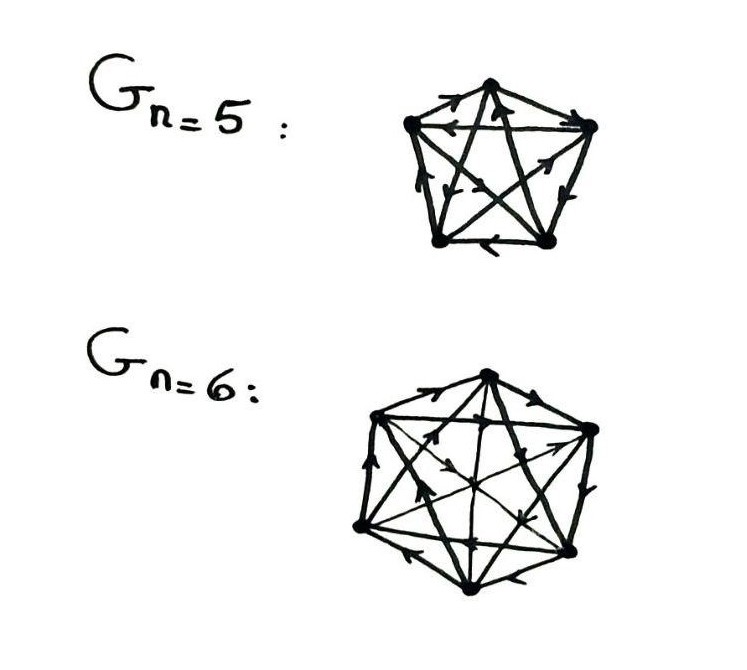
\includegraphics[height=5cm]{Graphw.jpg}}    
   
 
   $G_{n}$ را از روی 
    $G_{n-1}$ می‌سازیم به این صورت که  $G_{n-1}$ را جفت جفت افراز کرده و اتصال هر جفت با راس جدید را جداگانه بررسی می‌کنیم. جفت راس $i, j$ را در نظر بگیرید که در آن یال $i, j$ از سمت یال $i$ به سمت 
    $j$
     باشد، حال 
     (بدون کم شدن از کلیت مسئله)
      راس جدید
     $x$
      را به این صورت به مجموعه اضافه می‌کنیم:
    
       {\hspace*{6cm}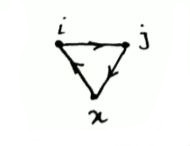
\includegraphics[height=2cm]{Graph2.jpg}}    
       
    تمام مسیر‌های
    $xj, xi, jx, ix, ij$ به طول حداکثر ۲ موجودند، این کار را برای تمام جفت راس‌ها انجام می‌دهیم. بنابراین تمام مسیر‌ها به طول حداکثر ۲ موجودند، راس $x$ به تمام راس‌ها یال دارد، پس به گراف دلخواه $G_{n}$ رسیدیم.
    
\notes
\Enote {n40}
ناقص بودن گام استقرا:
این گام در صورتی صحیح است که $n$ فرد باشد.
و با توجه به وابستگی اثبات $n$ های فرد به صحیح بودن حکم برای $n$ های زوج, حکم اثبات نمی شود.
\Tnote {n60}
حکم برای حالت ۱ و ۳ اثبات نشده است.
\solution*{پاسخ صحیح}


پایه استقرا:


   {\hspace*{5cm}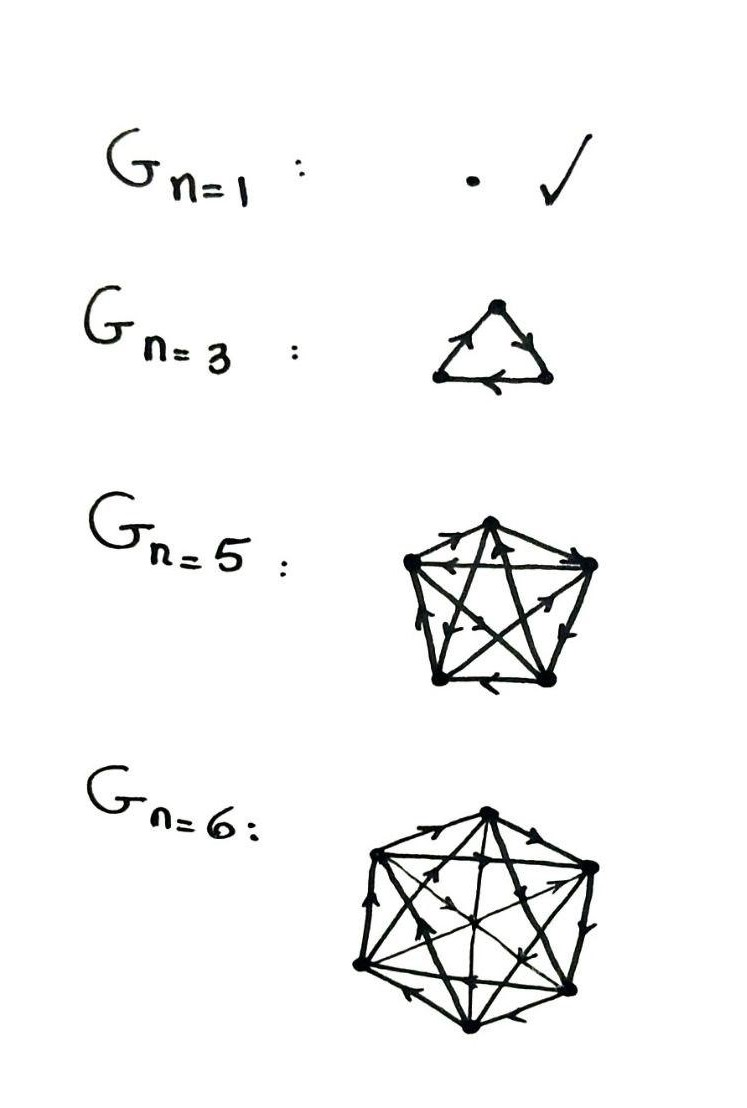
\includegraphics[height=5cm]{Graph1.jpg}}    
   
   برای $n>6$ ما دو حالت داریم: $\; \; \; \; \; \;$ حالت اول $n$ زوج
   .$\; \; \; \; \; \;$
   حالت دوم $n$ فرد.   
   
    الف ) $n$ فرد می‌باشد. پس
    $G_{n-1}$ تعداد زوجی راس دارد. $G_{n}$ را از روی 
    $G_{n-1}$ می‌سازیم به این صورت که  $G_{n-1}$ را جفت جفت افراز کرده و اتصال هر جفت با راس جدید را جداگانه بررسی می‌کنیم. جفت راس $i, j$ را در نظر بگیرید که در آن یال $i, j$ از سمت یال $i$ به سمت
     $j$   باشد، حال 
     (بدون کم شدن از کلیت مسئله)
      راس جدید
     $x$
      را به این صورت به مجموعه اضافه می‌کنیم:

    
       {\hspace*{6cm}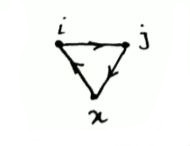
\includegraphics[height=2cm]{Graph2.jpg}}    
       
    تمام مسیر‌های
    $xj, xi, jx, ix, ij$ به طول حداکثر ۲ موجودند، این کار را برای تمام جفت راس‌ها انجام می‌دهیم. بنابراین تمام مسیر‌ها به طول حداکثر ۲ موجودند، راس $x$ به تمام راس‌ها یال دارد، پس به گراف دلخواه $G_{n}$ رسیدیم.
    
    ب) $n$ زوج باشد. در این حالت $G_{n}$ را از $G_{n-2}$ می‌سازیم. دو راس جدید $x, y$ را بهم متصل می‌کنیم(از $x$ به سمت $y$) حال به ازای هر راس $i$ در $G_{n-2}$ آن را به این صورت به $x$ به $y$ متصل می‌کنیم.
    
        {\hspace*{6cm}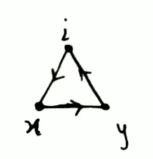
\includegraphics[height=2cm]{Graph3.jpg}}      
    
    تمامی مسیر‌های $iy, ix, yx, yi, xi, xy$ به طول حداکثر ۲ موجود هستند چون این کار را برای تمام راس‌های $G_{n-2}$ انجام دادیم پس تمام مسیرها به طول حداکثر ۲ موجودند و راس‌ها جدید $y, x$ به تمام راس‌ها یال دارند، پس گراف دلخواه $G_{n}$ را ساختیم.
    
    چون هم برای $n$های زوج ثابت کردیم و هم برای $n$ های فرد، پس می‌توان $G_{n}$ را به ازای تمام 
    $n>6$ ساخت.

%%%%%%%%%%%%%%%%%%%%%%%%%%%%%%%% question 4.3 %%%%%%%%%%%%%%%%%%%%%%%%%%%
\question

 نشان بدهید که میتوان اعداد $1,2,3,...,n$ را طوری کنار هم چید، که میانگین هیچ دو عددی بین آن دو عدد دیده نشود. 
 
 \solution
 برای $ n= 1 , 2$
 به طور بدیهی می‌توان جایگشتی ساخت که میانگین هیچ دو عددی بین آن دو عدد دیده نشود. 
 $$ n = 2 \rightarrow \{ 1, 2 \} $$
 برای n های بزرگ‌تر از ۲، عددها را به دو دسته زوج و فرد تقسیم می‌کنیم و اعداد را مانند الگوریتم زیر می‌چینیم.
 
 برای $ n=3 $ ابتدا اعداد فرد را در سمت چپ و سپس عدد زوج را می‌نویسیم. 
 $$ n=3 \rightarrow \{ 1, 3 ,2 \} $$
  
 برای $ n =4 $ نیز، دو دسته زوج و فرد را تشکیل می‌دهیم و مانند $ n =2 $ ، سمت چپ اعداد فرد و سمت راست اعداد زوج را می‌نویسیم.
 
 برای $ n = 5 $ نیز، دو دسته زوج و فرد را به ترتیب با ۲ و ۳ عضو تشکیل می‌دهیم و دسته فرد را سمت چپ و دسته زوج‌ را سمت راست قرار می‌دهیم.
 ‌ 
 
 اگر به همین ترتیب پیش برویم جایگشت مناسب برای هر عدد را می‌توان با استفاده از اعداد قبل نوشت. پس حکم اثبات شد.
 
  
 \notes
 \\%dont erase this :)
\\%dont erase this :)
 \refnote{n14} 
 
 
 مثال زدن و تعمیم دادن آن اثبات محسوب نمی‌شود.
 
 \Enote{n41}
 همین تفکر گام به گام را می‌توان با استفاده از استقرا بیان کرد. در این صورت باید همه الزامات استقرا اعم از پایه و فرض و حکم استقرا را نوشت و به طور کامل اثبات را پیش برد. در این پاسخ فقط پایه استقرا رعایت شده است. 
 
 
 \solution*{پاسخ صحیح} 
 
 پایه استقرا :$ n = 2 $  برقرار است.
 
 چینش: 2 1
 
 سوال را با دو گام حل می‌کنیم:
 
 آ) گام اول: $ n  \rightarrow  2n $
 
 ب) گام دوم: $ n \rightarrow n-1 $
 
 فرض استقرا: $ n = 2^k $ 
 
 حکم استقرا: $n = 2 ^ { k+1 } $ 
 
 
اثبات: مجموعه‌ی حکم را به دو قسمت زوج‌ها و فردها تقسیم می‌کنیم.
	\begin{enumerate}
		\item
برای زوج‌ها هر عدد را بر دو تقسیم می‌کنیم. به مجموعه‌ی فرض می‌رسیم که شرایط مسئله در آن برقرار است و جایگشتی از اعضا را دارد که در آن چینش میانگین هیچ دو عضوی بینشان نیست. حال این جایگشت را در نظر گرفته و هر عضو را در دو ضرب می‌کنیم.

 		\item

برای فردها هر عدد را به علاوه یک و سپس بر دو تقسیم می‌کنیم. به مجموعه‌ی فرض می‌رسیم که شرایط مسئله در آن برقرار است و جایگشتی از اعضا را دارد که در آن چینش میانگین هیچ دو عضوی بینشان نیست. حال
این جایگشت را در نظر گرفته و هر عضو را در دو ضرب  و منهای یک می‌کنیم.
 	\end{enumerate}
 	
 	
 	
ادعا می‌کنیم مجموعه‌ی حاصل مجموعه‌ی جواب است، هر دو عددی که از مجموعه‌ی زوج‌ها انتخاب کنیم ،میانگینشان هم فقط در دو ضرب شده است و در نتیجه بین آن دو نخواهد بود.
هر دو عددی که از مجموعه فردها انتخاب کنیم، میانگنشان در دو ضرب و منهای یک شده است و بنا به فرض بین آن دو نخواهد بود. اگر عددی از فردها و عددی از زوج‌ها را انتخاب کنیم، میانگینشان طبیعی نخواهد بود و جزو شرایط مسئله نیست.
همه‌ی حالت‌ها را بررسی کردیم، پس ادعا صحیح و حکم ثابت می‌شود.


با حذف بزرگ‌ترین عدد از مجموعه فرض استقرا می‌توان به جایگشتی از  $n-1 $ عضو رسید به ظوری که میانگین هیچ دو عضوی بینشان نیست. پس در این صورت شرایط سوال برای $n-1 $ برقرار است و حکم استقرا ثابت است. 


با شروع از پایه ۲ و با استفاده از گام اول می‌توان حکم را برای همه اعداد توان ۲ ثابت کرد و با استفاده از گام -۱ همه اعداد بین توان های ۲ متوالی را پوشش داد. بنابراین حکم سوال برای تمام اعداد طبیعی برقرار است. 



 \notes
 	
 \Enote{n42}
 	به این گونه سوالات که یک گام بزرگ (گام آ) دارد و یک گام معکوسی (گام ب) که کم می‌کند استقرای قهقرایی می‌گویند. در این سوالات حکم را با گام بزرگ اثبات می‌کنیم و با استفاده از گام کوچک از آن کم می‌کنیم تا همه اعداد را پوشش دهیم.
 	
\Enote{n43}
 	 توجه کنید در اثبات‌ها باید با استفاده از گام(ها) و فرض ، حکم را برای همه اعداد طبیعی ثابت کنید.
 	 
 	 
\chapter*{
نکات نوشتار}
\notes
\Nnote{n44}
در حل سوالات توجه کنید هر گزاره، فرمول، اتحاد و... که درستی آن‌ها اثبات شده است  باید منبع معتبر آن ‌ذکر شود‌. این منابع می‌توان اسم عام آن، آدرس سوال و تمرینی که قبلا داده شده، مطالب داخل کلاس، جزوه و... باشد. 

\Enote{n45}
در طول اثبات توصیه اکید می‌شود از کلمه «بدیهی است» استفاده نکنید. حتی در مسیر یافتن جواب هم در ذهن خود بسپارید هیج چیز بدیهی نیست، یا نیاز به اثبات دارد یا قبلا اثبات شده است یا از اصول و تعاریف پایه است 
\refnote{n44}.
به عبارتی برای هر جمله به سوال «چرا؟» پاسخ دهید.
چرا؟ :)
چون استفاده از بعضی از جملات اعم از «بدیهی است» و مواردی که اشاره خواهیم کرد در طول اثبات باعث کژفهمی کلیت اثبات یا کامل به نظر رسیدن اثباتی ناقص و یا حتی غلط می‌شود. 
به عبارت دیگر
مانند فرایند های منطقی
\refnote{n20}
هر جمله باید از جملات قبلی و یا اصول پایه نتیجه گرفته شود.

\Nnote{n45}
یکی از چراغ خطرهای در طول اثبات استفاده از «و .../و غیره/...» است. این کلمات به خودی خود بد نیستند، اما زمانی که ما می‌توانیم از علایم اختصاری استفاده کنیم اثبات ما تمیزتر و خواناتر و به طور حتم به دور از ابهام می‌شود.
برای شفاف شدن موضوع به دو مثال زیر توجه کنید:

\begin{enumerate}
\item
دنباله «۲و ۴و ۶و ...» را داریم.

«و ...» نشان دهنده چه جملاتی در دنباله است؟

آیا منظور دنباله $a_n =2n $ است؟

یا دنباله $a_n = a_{n-1} + a_{n-2} ,  a_0=2 , a_1=4$ ؟

یا دنباله $ a_n = 2n + (1-n)^3(2-n)^2(3-n) $ ؟ 
\item
s
را در نظر می‌گیریم $ a_1 + a_2 + ... + a_n $. 

زیباتر است بنویسیم :
$ s = \sum_{i=1}^{n} {a_i} $

\end{enumerate}

\Nnote{n46}
تا آن‌جا که می‌توانید جملات، عبارات ریاضی و گزاره‌ها را فارسی ننویسید. از گزاره‌های منطقی استفاده کنید یا به شکل عبارات و معادلات ریاضی بنویسید. در مباحثی که مدل نوشتاری خاص وجود دارد مثل استقرا و نظریه اعداد حتما اصول را رعایت کنید.

\Enote{n47}
از نوشتن عبارت هایی مثل "بهترین حالت این است که" یا "در بدترین حالت داریم که..." پرهیز کنید. توجه کنید که بهترین و بدترین و مفاهیمی از این دست, در ریاضیات معنایی ندارند مگر آن که آن‌ها را تعریف کنید و توضیح بدهید که چرا در نظر گرفتن این حالت به حل مسئله کمک می‌کند.

\Nnote{n48}
بهتر است در صورتی که در اثبات خود از روش یا ایده مشخص و شناخته شده‌ای استفاده می‌کنید, (مثل ناوردایی - استقرا - برهان خلف - دوگانه شماری و...)آن را ذکر کنید تا دنبال کردن اثبات شما برای خواننده راحت تر بشود و اثبات شما را بهتر متوجه بشود.

\Enote{n49}
اگر در نوشتن اثبات از رسم شکل استفاده می‌کنید, حذف کردن شکل نباید باعث ناقص شدن اثبات شما بشود, به عبارت دیگر شکل تنها باید به فهم بهتر اثبات کمک کند و نباید مستقیما برای اثبات استفاده شود.

\Enote{n50}
استفاده از مثال برای فهم بهتر اثبات یک حکم کلی اقدام خیلی خوبی است, اما نباید جایگزین اثبات اصلی بشود.

\chapter*{گراف}

\question
    ثابت کنید یک گراف ۳-منتظم رأس برشی دارد اگر و تنها اگر یال برشی داشته‌ باشد. 
 \solution 
 
 فرض کنید v یک راس برشی از گراف G است. چون گراف ۳-منتظم است پس با حذف v گراف به ۳ مولفه تقسیم می‌شود. همسایه‌های v را $ x, y, z  $ می‌نامیم. نشان می‌دهم هرکدام از یال‌ها برشی هستند.
 
 بدون تغییر کلیت سوال یال vx را در نظر بگیرید. مثالا v را در مولفه‌ای در نظر بگیرید که y در آن قرار دارد. می‌دانیم که x با تنها گذر از v می‌تواند به y برسد یعنی در واقع وارد مولفه مزبور شود. پس vx یال برشی است.
 
 برای طرف دوم می‌خواهیم ثابت کنیم؛ اگر گراف ۳-منتظم یال برشی داشته باشد، آنگاه راس برشی دارد.
 عکس نقیض گزاره فوق را در نظر می‌گیریم.
 
 عکس نقیض: اگر گراف ۳-منتظم راس برشی نداشته باشد، آنگاه یال برشی ندارد.
 
 در قسمت اول دیدیم اگر راس برشی داشته باشیم پس یال برشی داریم. بنابراین اگر راس برشی نداشته باشیم، یال برشی هم نداریم.
 
 عکس نقیض گزاره درست است. چون هر گزاره با عکس نقیض خود هم‌ارز است، پس گزاره اصلی هم درست است.
 
 \notes
 
 \Enote{n50}
 در حل سوالات باید تمامی حالت‌هابی که ممکن است پیش بیاید را در نظر بگیریم. در اینجا با حذف v ممکن است گراف به ۲ مولفه همبندی تقسیم شود.
 
 
 \refnote{n22}
 گزاره «اگر گراف ۳-منتظم راس برشی داشته باشد، آنگاه یال برشی دارد.» را معادل $p \rightarrow q $ در نظر بگیرید.
 
 گزاره «اگر گراف ۳-منتظم راس برشی نداشته باشد، آنگاه یال برشی ندارد.» معادل می‌شود با
 . $ \neg p \rightarrow \neg q $ 
 که این وارون گزاره فوق است و با هم هم‌ارز نیستند.
 بنابراین نمی‌توان از گر راس برشی داشته باشیم پس یال برشی داریم نتیجه بگیریم گر راس برشی نداشته باشیم، یال برشی هم نداریم. 
 \solution*{پاسخ صحیح} 
 
    ابتدا ثابت می‌کنیم که اگر در این گراف رأس برشی داشته باشیم، یال برشی داریم.
    
    اگر k رأس برشی باشد، چون درجه آن 3 است، دو حالت داریم : 
    
    1)	به دو مؤلفه یال داشته باشد. در این صورت به یکی از مؤلفه‌ها 2 یال و به دیگری یک یال دارد و می‎‌توانیم گراف را به صورت شکل 1 رسم کنیم. بدون کاسته شدن از کلیت مسئله، مولفه‌ای که k به آن یک یال دارد را A و مولفه دیگر را B می‌نامیم. چون k برشی است پس از A به B فقط یک مسیر گذرا از k وجود دارد و چون از A به k نیز فقط یک یال وجود دارد، این یال برشی است.
    
    2)	در غیر این صورت اگر به سه مؤلفه یال داشته باشد، به هریک از 3 مؤلفه، یک یال دارد و می‎توانیم گراف را به صورت شکل 2 رسم کنیم. چون k برشی است و به هر مؤلفه فقط یک یال دارد، پس هرکدام از این یال‌ها نیز برشی هستند. 
    
    
    
    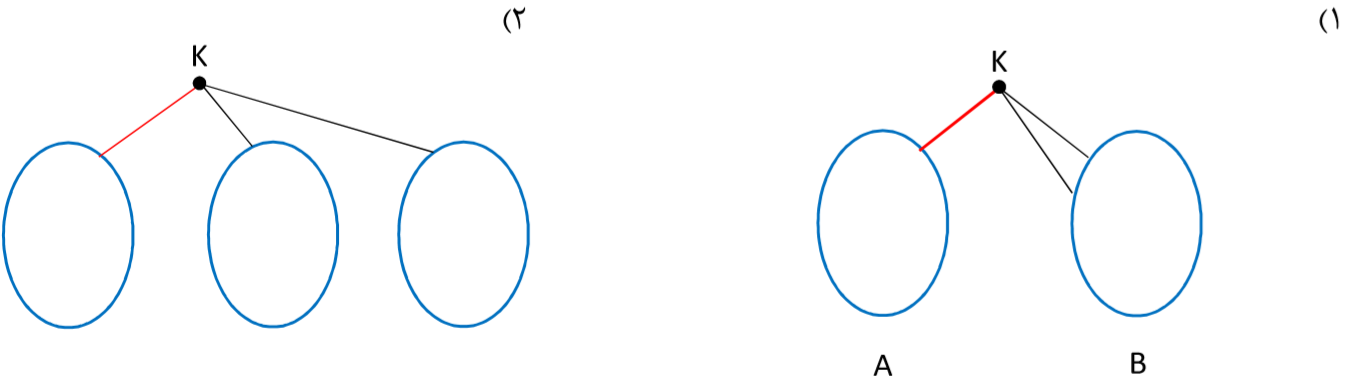
\includegraphics[width=15cm, height=3.5cm]{1.png}
   
   
    سپس اثبات می‎کنیم که اگر یال برشی داشته باشیم، رأس برشی داریم.
    
    اگر u یال برشی باشد، می‌توانیم گراف را مانند شکل زیر رسم کنیم و چون یال u برشی است، بنابراین به جز u یال دیگری از رأس a (یک سر یال u در یک مؤلفه) به مؤلفه دیگر وجود ندارد. بنابراین رأس a نیز برشی است.
    
    \leftline{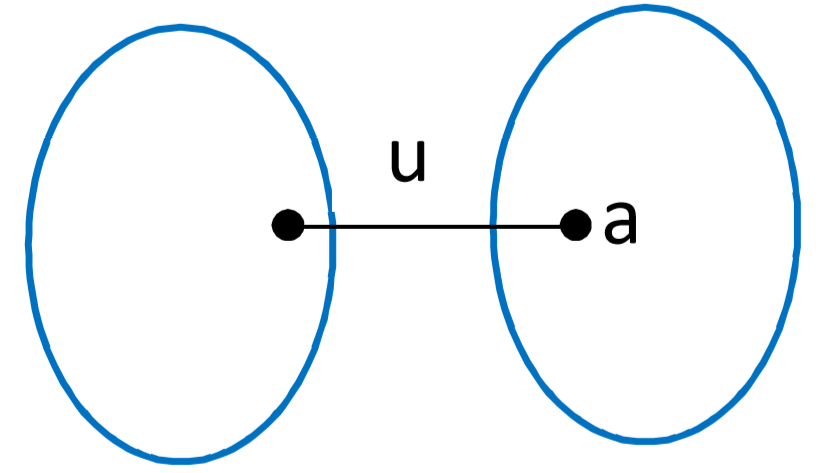
\includegraphics[width=3.3cm, height=2cm]{2.png}}
\end{document}